\documentclass[10pt]{article}
\usepackage[margin=0.9in]{geometry}
\usepackage[T1]{fontenc}
\usepackage{lmodern}
\usepackage{amsmath,amssymb}
\usepackage{graphicx}
\usepackage{booktabs}
\usepackage{multirow}
\usepackage{xcolor}
\usepackage[numbers,sort&compress]{natbib}
\usepackage[colorlinks=true,linkcolor=blue!50!black,citecolor=blue!50!black,urlcolor=blue!50!black]{hyperref}
\usepackage{tikz}
\usetikzlibrary{positioning,arrows.meta,fit,calc}
\usepackage{enumitem}
\setlist{nosep,leftmargin=*}
\usepackage{titlesec}
\titlespacing*{\section}{0pt}{7pt}{3pt}
\titlespacing*{\subsection}{0pt}{5pt}{2pt}
\setlength{\parskip}{2pt}

\newcommand{\R}{R}
\renewcommand{\Pr}{P}
% E6 (dilated oracle) results, filled in from outputs/results_dilated.jsonl
\newcommand{\EsixUa}{0.83}
\newcommand{\EsixPa}{0.07}
\newcommand{\EsixLa}{0.38}
\newcommand{\EsixBa}{0.33}
\newcommand{\EsixUb}{0.85}
\newcommand{\EsixPb}{0.12}
\newcommand{\EsixLb}{0.48}
\newcommand{\EsixBb}{0.44}
\newcommand{\EsixUc}{0.74}
\newcommand{\EsixPc}{0.01}
\newcommand{\EsixLc}{0.14}
\newcommand{\EsixBc}{0.11}
\newcommand{\EsixUd}{0.75}
\newcommand{\EsixPd}{0.02}
\newcommand{\EsixLd}{0.21}
\newcommand{\EsixBd}{0.15}
\newcommand{\EsixText}{%
\textbf{Result.} Growing the masks by one token closes most of the gap: at $K{=}144$, the dilated oracle's adversarial leakage (\EsixLc) is statistically indistinguishable from the learned score's
(difference $-0.03$, 95\% CI $[-0.06,+0.01]$), and at $K{=}288$ it falls from 0.49 to \EsixLa, though it remains above the learned score (difference $+0.08$, CI $[+0.05,+0.12]$).
So a large part of the leakage really comes from tokens \emph{adjacent} to the annotated regions, which confirms the context explanation.
Growing by two tokens is \emph{worse} than by one (\EsixLb\ at $K{=}288$). The reason is the budget. Two-token dilation flags 300 of 576 tokens per image on average,
and in 56\% of images more than $K{=}288$, so selection must keep some flagged tokens. Dilation gives the ring the same score as the core, so the selector cannot prefer ring tokens over core tokens.
The learned score is \emph{graded} (mean 0.89 inside a mask, 0.47 in the first ring, 0.34 in the second), so under a tight budget it gives up the least risky tokens first.
\emph{Lesson for the second half:} privacy risk should be a graded, context-aware score, not a binary region. This favours the learned head and motivates distance-weighted oracles such as $\Pr_i=\max_j \Pr^{GT}_j\,\gamma^{d(i,j)}$ as a stronger reference.}



\title{\vspace{-1.5em}\textbf{Useful but Not Revealing:}\\
Prompt-Conditioned, Privacy-Aware Visual Token Pruning for Vision-Language Models\\[2pt]
\large Mid-Term Report}
\author{Ahmed Abdelnaby}
\date{}

\begin{document}
\maketitle
\vspace{-2.5em}

\begin{abstract}
\noindent
Vision-language models (VLMs) pass hundreds of visual tokens to a large language model (LLM), including tokens that show faces, names or ID documents unrelated
to the user's question. We proposed to prune visual tokens by a score $S_i=\R_i-\lambda \Pr_i$ that rewards question relevance $\R_i$ and penalises privacy risk $\Pr_i$.
At mid-term, the full system is implemented on a frozen LLaVA-1.5-7B and evaluated on 200 VISPR-redactions test images (2,062 tasks) and 300 GQA questions,
at four token budgets, with oracle and learned privacy scores, and with three privacy metrics. Main findings so far:
(1) relevance-only pruning, the basis of existing token pruners, \emph{prefers} private tokens;
(2) a 0.27M-parameter privacy head on frozen CLIP features (token AP 0.87) cuts adversarial attribute leakage from 0.72 to 0.54 at 50\% of the tokens with no loss of GQA accuracy;
(3) the learned score leaks \emph{less} than the ground-truth masks, because it also covers context tokens around the annotated regions;
(4) removing tokens does not remove information: private attributes remain linearly recoverable from the kept tokens.
These findings shift the second half of the project from ``tune $\lambda$'' to ``remove context leakage'' and ``fix weak text attributes''.
\end{abstract}

\section{Problem and Motivation (updated)}
Given an image $I$ and question $q$, LLaVA-1.5~\cite{liu2024llava15} encodes $I$ into $N{=}576$ visual tokens (a $24{\times}24$ grid of CLIP~\cite{radford2021clip} patches)
and conditions the LLM on all of them. We ask: \emph{can we choose $K<N$ tokens that keep what is needed to answer $q$ while withholding privacy-sensitive content?}
This matters because personal photos routinely contain private attributes~\cite{orekondy2017vispr}; VLMs infer such attributes at scale~\cite{tomekce2024private};
split device/cloud inference sends every visual token to a server; and token pruning is already used for efficiency~\cite{chen2024fastv,zhang2025sparsevlm,zhang2025vispruner,alvar2025divprune},
so making it privacy-aware costs nothing at inference. Pixel obfuscation is known to be defeatable~\cite{mcpherson2016defeating}; whether \emph{token} removal is a sound form of redaction was untested.

\textbf{What changed since the proposal.} The hypothesis that useful tokens and private tokens are largely disjoint is \emph{partly} supported:
at a 50\% budget, utility is unaffected while geometric privacy improves sharply. The proposal underestimated one effect. Information about
a private region is spread into its neighbours by the 24 self-attention layers of the vision encoder, so a correct mask of the private region is not enough.
The research question for the second half is therefore sharper: \emph{how much of a VLM's private-attribute leakage is located in the private region itself, and how much in its context?}

\section{Related Work (updated)}
\textbf{Visual-token reduction.} FastV~\cite{chen2024fastv} prunes low-attention image tokens after layer 2; SparseVLM~\cite{zhang2025sparsevlm} scores tokens with the text;
VisPruner~\cite{zhang2025vispruner} argues text--visual attention is unreliable and uses visual cues; DivPrune~\cite{alvar2025divprune} maximises diversity; ToMe~\cite{bolya2023tome} merges tokens inside the ViT.
All optimise efficiency and utility only. Our results add a new observation about them: attention-based relevance ranks people and text highly, so such pruners retain private content \emph{preferentially}.
\textbf{Visual privacy.} VISPR~\cite{orekondy2017vispr} defines image privacy attributes, and VISPR-redactions~\cite{orekondy2018redactions} provides pixel masks and shows that redacting them gives privacy at little utility cost \emph{for human viewers}.
We study redaction for a \emph{model}, conditioned on the question, and find that it behaves differently: masks that suffice for humans leave private attributes recoverable by the model.
\textbf{Dense CLIP features.} Our CLIP relevance uses MaskCLIP value features~\cite{zhou2022maskclip}; the attention-sink tokens described for ViTs~\cite{darcet2024registers} motivated our rank normalisation.

\section{Updated Technical Plan}
\begin{figure}[t]
\centering
\resizebox{0.92\linewidth}{!}{%
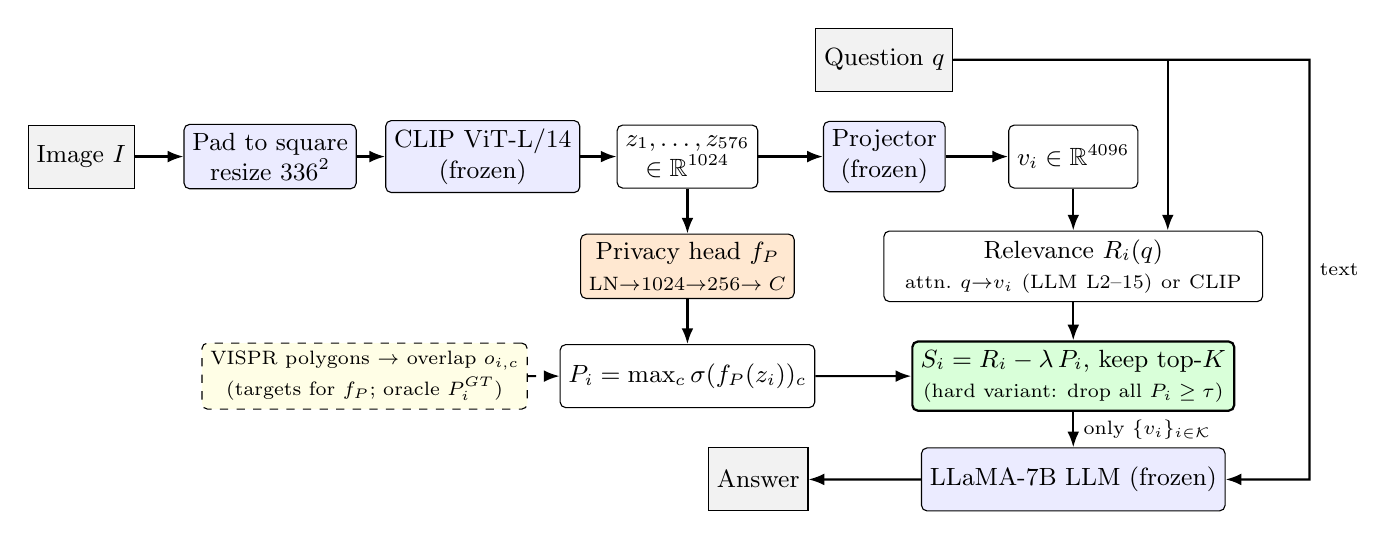
\begin{tikzpicture}[yscale=0.82,
  node distance=5mm and 7mm,
  box/.style={draw,rounded corners=2pt,align=center,font=\small,minimum height=8mm,inner sep=3pt},
  frozen/.style={box,fill=blue!8},
  train/.style={box,fill=orange!18},
  ours/.style={box,fill=green!15,thick},
  io/.style={box,fill=gray!10,sharp corners},
  arr/.style={-{Latex[length=2mm]},thick}]
% row 1: vision path
\node[io]     (img)  at (0,0)    {Image $I$};
\node[frozen] (pad)  at (2.4,0)  {Pad to square\\resize $336^2$};
\node[frozen] (vit)  at (5.1,0)  {CLIP ViT-L/14\\(frozen)};
\node[box]    (z)    at (7.7,0)  {$z_1,\dots,z_{576}$\\$\in\mathbb{R}^{1024}$};
\node[frozen] (proj) at (10.2,0) {Projector\\(frozen)};
\node[box]    (v)    at (12.6,0) {$v_i\in\mathbb{R}^{4096}$};
\node[io]     (q)    at (10.2,1.5) {Question $q$};
% row 2: scoring
\node[train]  (ph)   at (7.7,-1.7) {Privacy head $f_P$\\\scriptsize LN$\to$1024$\to$256$\to C$};
\node[box,text width=46mm] (R) at (12.6,-1.7) {Relevance $\R_i(q)$\\\scriptsize attn.\ $q{\to}v_i$ (LLM L2--15) or CLIP};
% row 3: selection and answer
\node[box,dashed,fill=yellow!10] (gt) at (3.6,-3.4) {\scriptsize VISPR polygons $\to$ overlap $o_{i,c}$\\\scriptsize (targets for $f_P$; oracle $\Pr^{GT}_i$)};
\node[box]    (P)    at (7.7,-3.4) {$\Pr_i=\max_c \sigma(f_P(z_i))_c$};
\node[ours]   (S)    at (12.6,-3.4) {$S_i=\R_i-\lambda\,\Pr_i$, keep top-$K$\\\scriptsize (hard variant: drop all $\Pr_i\ge\tau$)};
\node[frozen] (llm)  at (12.6,-5.0) {LLaMA-7B LLM (frozen)};
\node[io]     (ans)  at (8.6,-5.0) {Answer};
\draw[arr] (img)--(pad); \draw[arr] (pad)--(vit); \draw[arr] (vit)--(z); \draw[arr] (z)--(proj); \draw[arr] (proj)--(v);
\draw[arr] (z)--(ph); \draw[arr] (ph)--(P); \draw[arr] (v)--(R); \draw[arr] (R)--(S);
\draw[arr] (q.east)-|([xshift=12mm]R.north);
\draw[arr] (q.east)-|(15.6,-5.0) node[pos=0.75,right,font=\scriptsize]{text}--(llm.east);
\draw[arr] (P)--(S);
\draw[arr] (S)--(llm) node[midway,right,font=\scriptsize]{only $\{v_i\}_{i\in\mathcal K}$};
\draw[arr] (llm)--(ans);
\draw[arr,dashed] (gt)--(P);
\end{tikzpicture}
}
\caption{Pipeline (unchanged from the proposal). Blue: frozen LLaVA-1.5. Orange: the only trained module (${\approx}0.27$M parameters). Green: privacy-aware selection.
The LLM receives only the $K$ selected visual tokens, in raster order.}
\label{fig:arch}
\vspace{-0.5em}
\end{figure}

The method is the one proposed (Fig.~\ref{fig:arch}); we summarise it and mark the changes.
\textbf{Model.} Frozen LLaVA-1.5-7B. Images are padded to a square and resized to $336^2$ (we disable the Hugging Face processor's default centre crop, which silently cut image content and misaligned the masks).
We build the LLM input \texttt{[prefix | $v_i$, $i\in\mathcal K$ | question]} ourselves; with $\mathcal K$ = all tokens this reproduces the reference implementation exactly (max logit difference 0.0).

\textbf{Privacy risk $\Pr_i$.} Oracle: $\Pr^{GT}_i=|A_i\cap\bigcup_c M_c|/|A_i|$, the share of token $i$'s $14{\times}14$ patch $A_i$ covered by any VISPR-redactions polygon $M_c$ after the same pad-and-resize
(28 attributes; 28.7\% of test tokens have $\Pr^{GT}_i>0.25$). Learned: $\Pr_i=\max_c\sigma(f_P(z_i))_c$ with $f_P$ = LayerNorm$\to$Linear(1024,256)$\to$GELU$\to$Linear(256,28) on the frozen CLIP feature $z_i$,
trained on soft per-class overlaps with class-weighted BCE ($w^+_c=\min(\text{neg}_c/\text{pos}_c,100)$) for 15 epochs, model selection on validation token AP.

\textbf{Relevance $\R_i$.} R1 (main): mean attention from question tokens to visual token $i$ over LLM layers 2--15 and all heads. R2 (deployable): cosine similarity between CLIP's text embedding of $q$ and MaskCLIP patch features; it needs no LLM pass.
R3 (oracle): leave-$2{\times}2$-block-out log-likelihood drop of the full-image answer. All are rank-normalised to $[0,1]$.

\textbf{Selection.} Keep the top-$K$ of $S_i=\R_i-\lambda\Pr_i$ (soft; the exact solution of $\max_x\sum_i x_i(\R_i-\lambda\Pr_i)$ s.t.\ $\sum_i x_i=K$),
or never keep $\Pr_i\ge\tau$ (hard; keeps $\le K$ tokens).

\textbf{Changes to the plan, and why.}
\begin{enumerate}
\item \emph{Learned $\Pr$ is now the primary privacy score, not just a stand-in for the oracle.} It leaks less than the oracle (Sec.~\ref{sec:context}); the oracle is kept as a geometric reference.
\item \emph{New experiment E6: dilated oracle masks.} To test \emph{why} the learned score wins, we grow $\Pr^{GT}$ by $r\in\{1,2\}$ tokens (grey-scale dilation on the $24{\times}24$ grid) and re-run selection. Run for this report.
\item \emph{New direction: in-encoder redaction.} Because of context leakage, the second half adds pruning or attention-masking \emph{inside} the CLIP ViT (blocking attention to tokens with high $\Pr_i$ from layer $\ell$ on), which prevents private content from spreading rather than deleting it afterwards.
\item \emph{New direction: text-aware privacy.} The head is weak on text attributes (AP 0.07--0.39 for username, e-mail, address, name), and those attributes leak most. We will add text-region features (e.g.\ an OCR detector's boxes) as extra head inputs.
\item \emph{Utility evaluation.} Easy VISPR neutral questions barely separate methods (random keeps 0.86 agreement at 50\%), so GQA testdev~\cite{hudson2019gqa} accuracy is now the primary utility metric, and low budgets (25\%, 10\%) are the main operating points.
\item \emph{Deferred.} R3 (leave-block-out) costs about 144 forward passes per question; it is limited to a 30-image subset. Cross-dataset generalisation moves to the last phase.
\end{enumerate}

\section{Intermediate Results}
\textbf{Setup.} VISPR-redactions splits: 3,873 / 1,611 / 2,989 train/val/test images; the head is trained on train and selected on val. Evaluation uses 200 random test images:
600 privacy-neutral utility questions, 531 adversarial probes (official VISPR yes/no question for a \emph{present} attribute, with tokens selected using the probe as $q$),
531 benign probes (same probe, tokens selected for a neutral question), and 400 absent-attribute probes (false-``yes'' control), plus 300 GQA testdev-balanced questions.
Budgets $K\in\{58,144,288,432\}$; $\lambda\in\{0.1,\dots,2\}$; $\tau\in\{0.5,0.8\}$; greedy decoding. One RTX 4090; about 40\,s per image for the full grid.
Metrics: PTR $=\sum_i x_i\Pr^{GT}_i/\sum_i\Pr^{GT}_i$; leakage = ``yes'' rate on present-attribute probes; recoverability = mAP of a linear probe predicting the 28 attributes from the mean of the kept tokens.

\subsection{The privacy head}
\begin{figure}[h]
\centering
\includegraphics[width=0.95\linewidth]{figs/mask_check.png}
\vspace{-1.2em}
\caption{Token-level privacy ground truth $\Pr^{GT}_i$ (red) on random test images after LLaVA's pad-and-resize; titles list the annotated attributes.}
\label{fig:masks}
\vspace{-0.8em}
\end{figure}
Token AP for ``private vs.\ not'' is 0.87 on test (val 0.86); mean per-class AP is 0.48. Per-class quality is very uneven (Table~\ref{tab:head}): large visual categories are detected well, text-based ones poorly.
This is expected, since 14-pixel CLIP patches do not resolve characters, and it explains the per-attribute leakage pattern below.

\begin{table}[h]
\centering\small
\setlength{\tabcolsep}{4pt}
\begin{tabular}{@{}lc lc lc lc@{}}
\toprule
attribute & AP & attribute & AP & attribute & AP & attribute & AP \\
\midrule
person & 0.91 & ticket & 0.78 & nudity & 0.61 & name & 0.39 \\
face & 0.88 & handwriting & 0.76 & license plate & 0.49 & address & 0.29 \\
passport & 0.84 & credit card & 0.73 & date/time & 0.47 & e-mail & 0.13 \\
\bottomrule
\end{tabular}
\caption{Token-level AP of the learned head per attribute (test set, selected classes). Text attributes are the weak spot.}
\label{tab:head}
\vspace{-1em}
\end{table}

\subsection{Main results}
\begin{table}[t]
\centering\small
\setlength{\tabcolsep}{4pt}
\begin{tabular}{@{}clcccccc@{}}
\toprule
$K$ & Method (attention $\R$) & VISPR util.$\uparrow$ & GQA acc.$\uparrow$ & PTR$\downarrow$ & Adv.\ leak$\downarrow$ & Benign leak$\downarrow$ & Recover.\ mAP$\downarrow$ \\
\midrule
576 & Full & 1.00 & 0.600 & 1.00 & 0.79 & 0.79 & 0.81 \\
\midrule
\multirow{6}{*}{288} & Random & 0.86 & 0.583 & 0.49 & 0.72 & 0.72 & 0.80 \\
 & Relevance only ($\lambda{=}0$) & 0.87 & 0.600 & 0.66 & 0.72 & 0.72 & 0.79 \\
 & Soft, oracle $\Pr^{GT}$, $\lambda{=}2$ & 0.86 & -- & 0.07 & 0.49 & 0.44 & 0.69 \\
 & Soft, learned $\Pr$, $\lambda{=}1$ & 0.87 & 0.600 & 0.20 & 0.54 & 0.47 & 0.71 \\
 & Soft, learned $\Pr$, $\lambda{=}2$ & 0.84 & 0.557 & 0.13 & 0.30 & 0.27 & 0.68 \\
 & Hard, learned $\Pr$, $\tau{=}0.5$ ($\bar K{=}239$) & 0.74 & 0.560 & 0.07 & 0.05 & 0.05 & 0.54 \\
\midrule
\multirow{5}{*}{144} & Random & 0.79 & 0.560 & 0.25 & 0.63 & 0.63 & 0.76 \\
 & Relevance only & 0.85 & 0.577 & 0.32 & 0.75 & 0.66 & 0.77 \\
 & Soft, oracle $\Pr^{GT}$, $\lambda{=}2$ & 0.79 & -- & 0.01 & 0.35 & 0.28 & 0.65 \\
 & Soft, learned $\Pr$, $\lambda{=}1$ & 0.82 & 0.540 & 0.05 & 0.29 & 0.20 & 0.64 \\
 & Soft, learned $\Pr$, $\lambda{=}2$ & 0.77 & 0.550 & 0.04 & 0.17 & 0.10 & 0.59 \\
\bottomrule
\end{tabular}
\caption{Results on 200 VISPR test images and 300 GQA questions. Utility is agreement with the full-token answer. Absent-attribute false-``yes'' rate is $\le 0.10$ for every configuration, so leakage is not a ``yes'' bias.
Oracle masks do not exist for GQA images.}
\label{tab:main}
\vspace{-0.8em}
\end{table}

\begin{figure}[t]
\centering
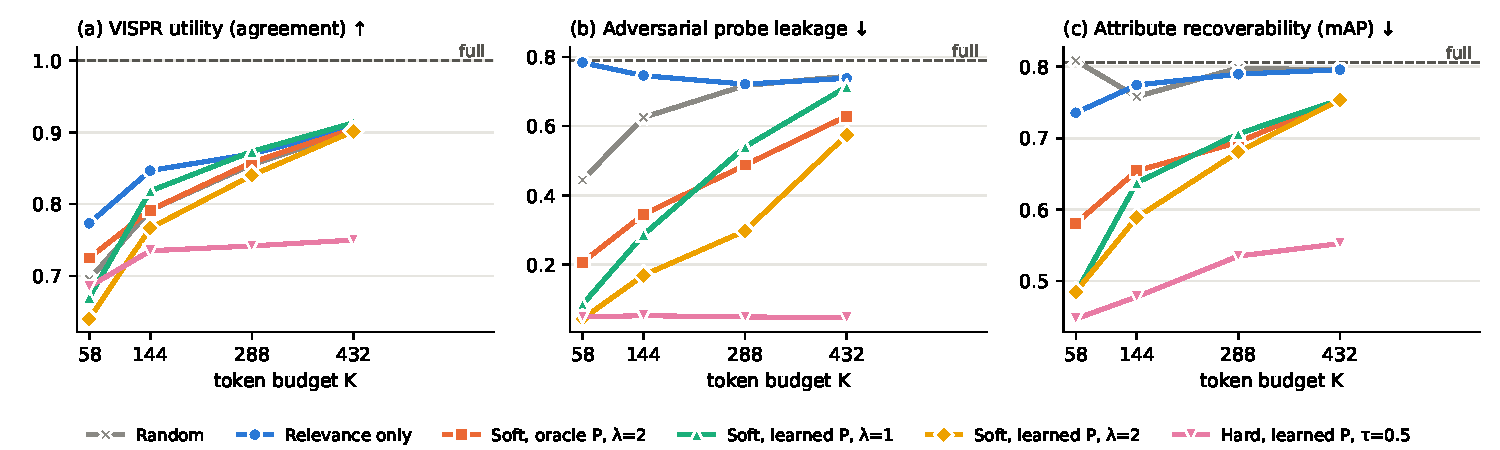
\includegraphics[width=\linewidth]{figs/budget_curves.pdf}
\vspace{-1.6em}
\caption{Utility, adversarial leakage and recoverability across token budgets (attention relevance). The hard gate keeps fewer than $K$ tokens.
Privacy-aware selection moves leakage far below relevance-only pruning at every budget; recoverability falls much less.}
\label{fig:budget}
\vspace{-0.8em}
\end{figure}

Table~\ref{tab:main} and Fig.~\ref{fig:budget} summarise E1 (oracle $\Pr$) and E3 (learned $\Pr$). Paired bootstrap 95\% intervals (2,000 resamples, same tasks) for the key differences at $K{=}288$ are in Table~\ref{tab:ci}.

\begin{table}[h]
\centering\small
\begin{tabular}{@{}llcc@{}}
\toprule
Comparison at $K{=}288$ & Metric & Difference & 95\% CI \\
\midrule
learned $\lambda{=}1$ $-$ relevance only & GQA accuracy & $+0.000$ & $[-0.030,+0.030]$ \\
learned $\lambda{=}1$ $-$ relevance only & adversarial leakage & $-0.181$ & $[-0.217,-0.143]$ \\
learned $\lambda{=}2$ $-$ relevance only & adversarial leakage & $-0.424$ & $[-0.467,-0.382]$ \\
learned $\lambda{=}2$ $-$ relevance only & GQA accuracy & $-0.043$ & $[-0.080,-0.007]$ \\
learned $\lambda{=}2$ $-$ oracle $\lambda{=}2$ & adversarial leakage & $-0.190$ & $[-0.230,-0.153]$ \\
\bottomrule
\end{tabular}
\caption{Paired bootstrap confidence intervals.}
\label{tab:ci}
\vspace{-1em}
\end{table}

\textbf{Observation 1: relevance-based pruning prefers private content.} Relevance-only pruning keeps \emph{more} private tokens than random (PTR 0.66 vs.\ 0.49 at $K{=}288$), and at $K{=}58$ its adversarial leakage (0.78) is almost that of the full model, while random's is 0.44.
LLaVA's attention concentrates on people and text, which is exactly where VISPR's attributes are. Attention-based efficiency pruners, as used in prior work, would therefore act as \emph{privacy-amplifying} filters.

\textbf{Observation 2: privacy can be bought cheaply at moderate budgets.} With learned $\Pr$ and $\lambda{=}1$ at $K{=}288$, GQA accuracy is unchanged (CI includes 0), PTR falls from 0.66 to 0.20, and leakage falls by 0.18.
$\lambda{=}2$ halves leakage again for a small, significant 4-point GQA cost. At $K{=}144$ the trade-off is still favourable for leakage, but the GQA cost grows to 2--4 points.
The hard gate gives near-zero leakage (0.05 at every budget) but costs 13 points of VISPR agreement, because it removes every high-risk token regardless of the question.

\textbf{Observation 3: removing tokens does not remove information.} With the oracle at $\lambda{=}2$, only 7\% of private tokens survive, yet the model still confirms 49\% of present attributes,
and a linear probe recovers attributes with mAP 0.69 (full model 0.81; chance level, the mean attribute prevalence, is 0.09). Even the hard gate leaves recoverability at 0.54, six times chance.
CLIP's self-attention has already copied information about the private regions into neighbouring tokens before any pruning happens.

\subsection{Why the learned score beats the oracle: context tokens}\label{sec:context}
The learned head flags more tokens than the masks (239 vs.\ 166 per image at threshold 0.5), and 36\% of its high-risk tokens lie \emph{outside} the masks. These tokens are concentrated next to the masks:
the probability that a token is flagged is 0.93 inside a mask, 0.43 in the first ring of tokens around it, 0.27 in the second ring, and 0.15 further away.
The head, which sees contextual CLIP features, has learned that the neighbours of a face also ``contain'' the face.

\textbf{E6, dilated oracle (new).} If context explains the gap, growing the oracle masks should close it. Table~\ref{tab:dil} reports the result at the same budgets and $\lambda$.

\begin{table}[h]
\centering\small
\begin{tabular}{@{}clcccc@{}}
\toprule
$K$ & Privacy score ($\lambda{=}2$, attention $\R$) & VISPR util.$\uparrow$ & PTR$\downarrow$ & Adv.\ leak$\downarrow$ & Benign leak$\downarrow$ \\
\midrule
\multirow{4}{*}{288} & Oracle $\Pr^{GT}$ & 0.86 & 0.07 & 0.49 & 0.44 \\
 & Oracle dilated by 1 token & \EsixUa & \EsixPa & \EsixLa & \EsixBa \\
 & Oracle dilated by 2 tokens & \EsixUb & \EsixPb & \EsixLb & \EsixBb \\
 & Learned $\Pr$ & 0.84 & 0.13 & 0.30 & 0.27 \\
\midrule
\multirow{4}{*}{144} & Oracle $\Pr^{GT}$ & 0.79 & 0.01 & 0.35 & 0.28 \\
 & Oracle dilated by 1 token & \EsixUc & \EsixPc & \EsixLc & \EsixBc \\
 & Oracle dilated by 2 tokens & \EsixUd & \EsixPd & \EsixLd & \EsixBd \\
 & Learned $\Pr$ & 0.77 & 0.04 & 0.17 & 0.10 \\
\bottomrule
\end{tabular}
\caption{E6: dilating the oracle masks. PTR is always measured against the undilated masks.}
\label{tab:dil}
\vspace{-1em}
\end{table}

\EsixText

\subsection{Which attributes leak, and deployable relevance}
\textbf{Per attribute} (adversarial leakage at $K{=}288$, full $\to$ learned $\lambda{=}2$): face 0.84$\to$0.10, person 0.96$\to$0.27, nudity 0.48$\to$0.09, name 0.76$\to$0.35, date/time 0.86$\to$0.53, handwriting 1.00$\to$0.71.
Visual attributes are suppressed; text attributes persist, matching the head's weak AP on text (Table~\ref{tab:head}). The oracle is much worse than the learned score on \emph{person} (0.69 vs.\ 0.27):
a person is recognisable from context such as clothing, shadows and posture, which lies outside a tight polygon.

\textbf{E4, CLIP relevance (deployable under split inference).} With CLIP relevance, which needs no LLM pass, GQA accuracy behaves like attention relevance (0.600 for relevance only at $K{=}288$; 0.563 with learned $\lambda{=}1$),
but VISPR agreement is about 7 points lower (0.80 vs.\ 0.87), because CLIP similarity is a weak localiser for generic questions such as ``describe the scene''.
Its benign leakage is lower (0.16 vs.\ 0.47 at learned $\lambda{=}1$), because CLIP relevance does not chase people the way LLM attention does.

\subsection{Lessons from implementation}
\textbf{Normalisation matters:} a few ``sink'' visual tokens receive far more attention than the rest~\cite{darcet2024registers}, so min--max scaling compresses most $\R_i$ towards 0 and changes the effective strength of $\lambda$ from image to image; rank normalisation gives $\lambda$ the same meaning everywhere (a min--max ablation is planned).
\textbf{Preprocessing must match the labels:} the default centre crop of the Hugging Face processor cuts off part of non-square images and misaligns the masks, a silent error that a visual check of the masks (Fig.~\ref{fig:masks}) catches immediately.
\textbf{Batching:} generating one answer per configuration (about 125 per question) is the bottleneck; batching equal-length keep-sets makes it feasible, and capping a batch at 8K visual tokens removed out-of-memory failures (de-duplicating identical keep-sets saves only 12\%).
\textbf{Infrastructure:} intermittent ``impossible'' Python errors were traced to one faulty CPU core of the workstation; all reported runs were pinned to the healthy cores.

\section{Future Work}
\textbf{Remaining plan.}
\begin{enumerate}
\item \emph{In-encoder redaction (weeks 1--2).} Mask attention \emph{to} high-$\Pr$ tokens in the CLIP ViT from layer $\ell\in\{4,8,12,16\}$ onward, so that private content cannot spread; $\Pr$ is computed from an early layer. Success criterion: recoverability at $K{=}288$ below 0.60 with no GQA loss.
\item \emph{Graded oracle (week 1).} Replace the binary dilation of E6 with a distance-decayed oracle and re-test whether any oracle can match the learned score.
\item \emph{Text-aware privacy head (week 2).} Add text-detector box features to $f_P$ and evaluate per-class AP and leakage on name, address, date/time and handwriting.
\item \emph{Stronger privacy probes (week 3).} Current probes test detection (``is a face visible?''). We will add extraction probes (``what is the name on the card?'', ``read the license plate''), scored by string match against OCR ground truth.
\item \emph{Oracle relevance R3 and pruner baselines (week 3).} Leave-block-out on 30 images as the upper bound; FastV and DivPrune as alternative $\R$.
\item \emph{Scale and generalise (week 4).} All 2,989 test images for the final configurations; a second VLM (e.g.\ a newer LLaVA variant) to check that observations 1--3 are not LLaVA-1.5-specific; a second privacy dataset.
\item \emph{Final report (weeks 5--6).}
\end{enumerate}
\textbf{Risks.} In-encoder masking changes the features the LLM was trained on, which may cost more utility than pruning; we will compare at matched leakage.
Extraction probes need OCR ground truth that VISPR-redactions provides only for some attributes; we will restrict them to those.

\section{Limitations of the Current Results}
(i) Leakage probes measure whether the model \emph{notices} an attribute, a weaker notion than extraction (addressed in future work item 3).
(ii) The evaluation uses 200 images and one model; the main differences are statistically significant at this size (Table~\ref{tab:ci}), but generality is unverified.
(iii) The hard gate keeps fewer tokens than $K$, so it is compared at a slightly lower budget.
(iv) VISPR utility questions are generated, not human-written; GQA is therefore the primary utility measure.

{\footnotesize
\setlength{\bibsep}{1pt}
\bibliographystyle{abbrvnat}
\bibliography{refs}
}
\end{document}
